\section{实证结果分析}

\subsection{RGARCH-CARR-SK 动态压力风险结果}

本节首先考察 MarketLSI 压力风险是否具有可度量的动态聚集特征。若 MarketLSI 仅为短期噪声，则条件压力风险路径不应在高压力阶段持续抬升；反之，若其包含市场状态信息，则条件压力风险应在 MarketLSI 局部高值附近同步上行。

为检验这一点，图 \ref{fig:rgarch-risk} 报告 RGARCH-CARR-SK 估计得到的条件压力风险 \(\lambda_t\) 路径。

\begin{figure}[!htbp]
    \centering
    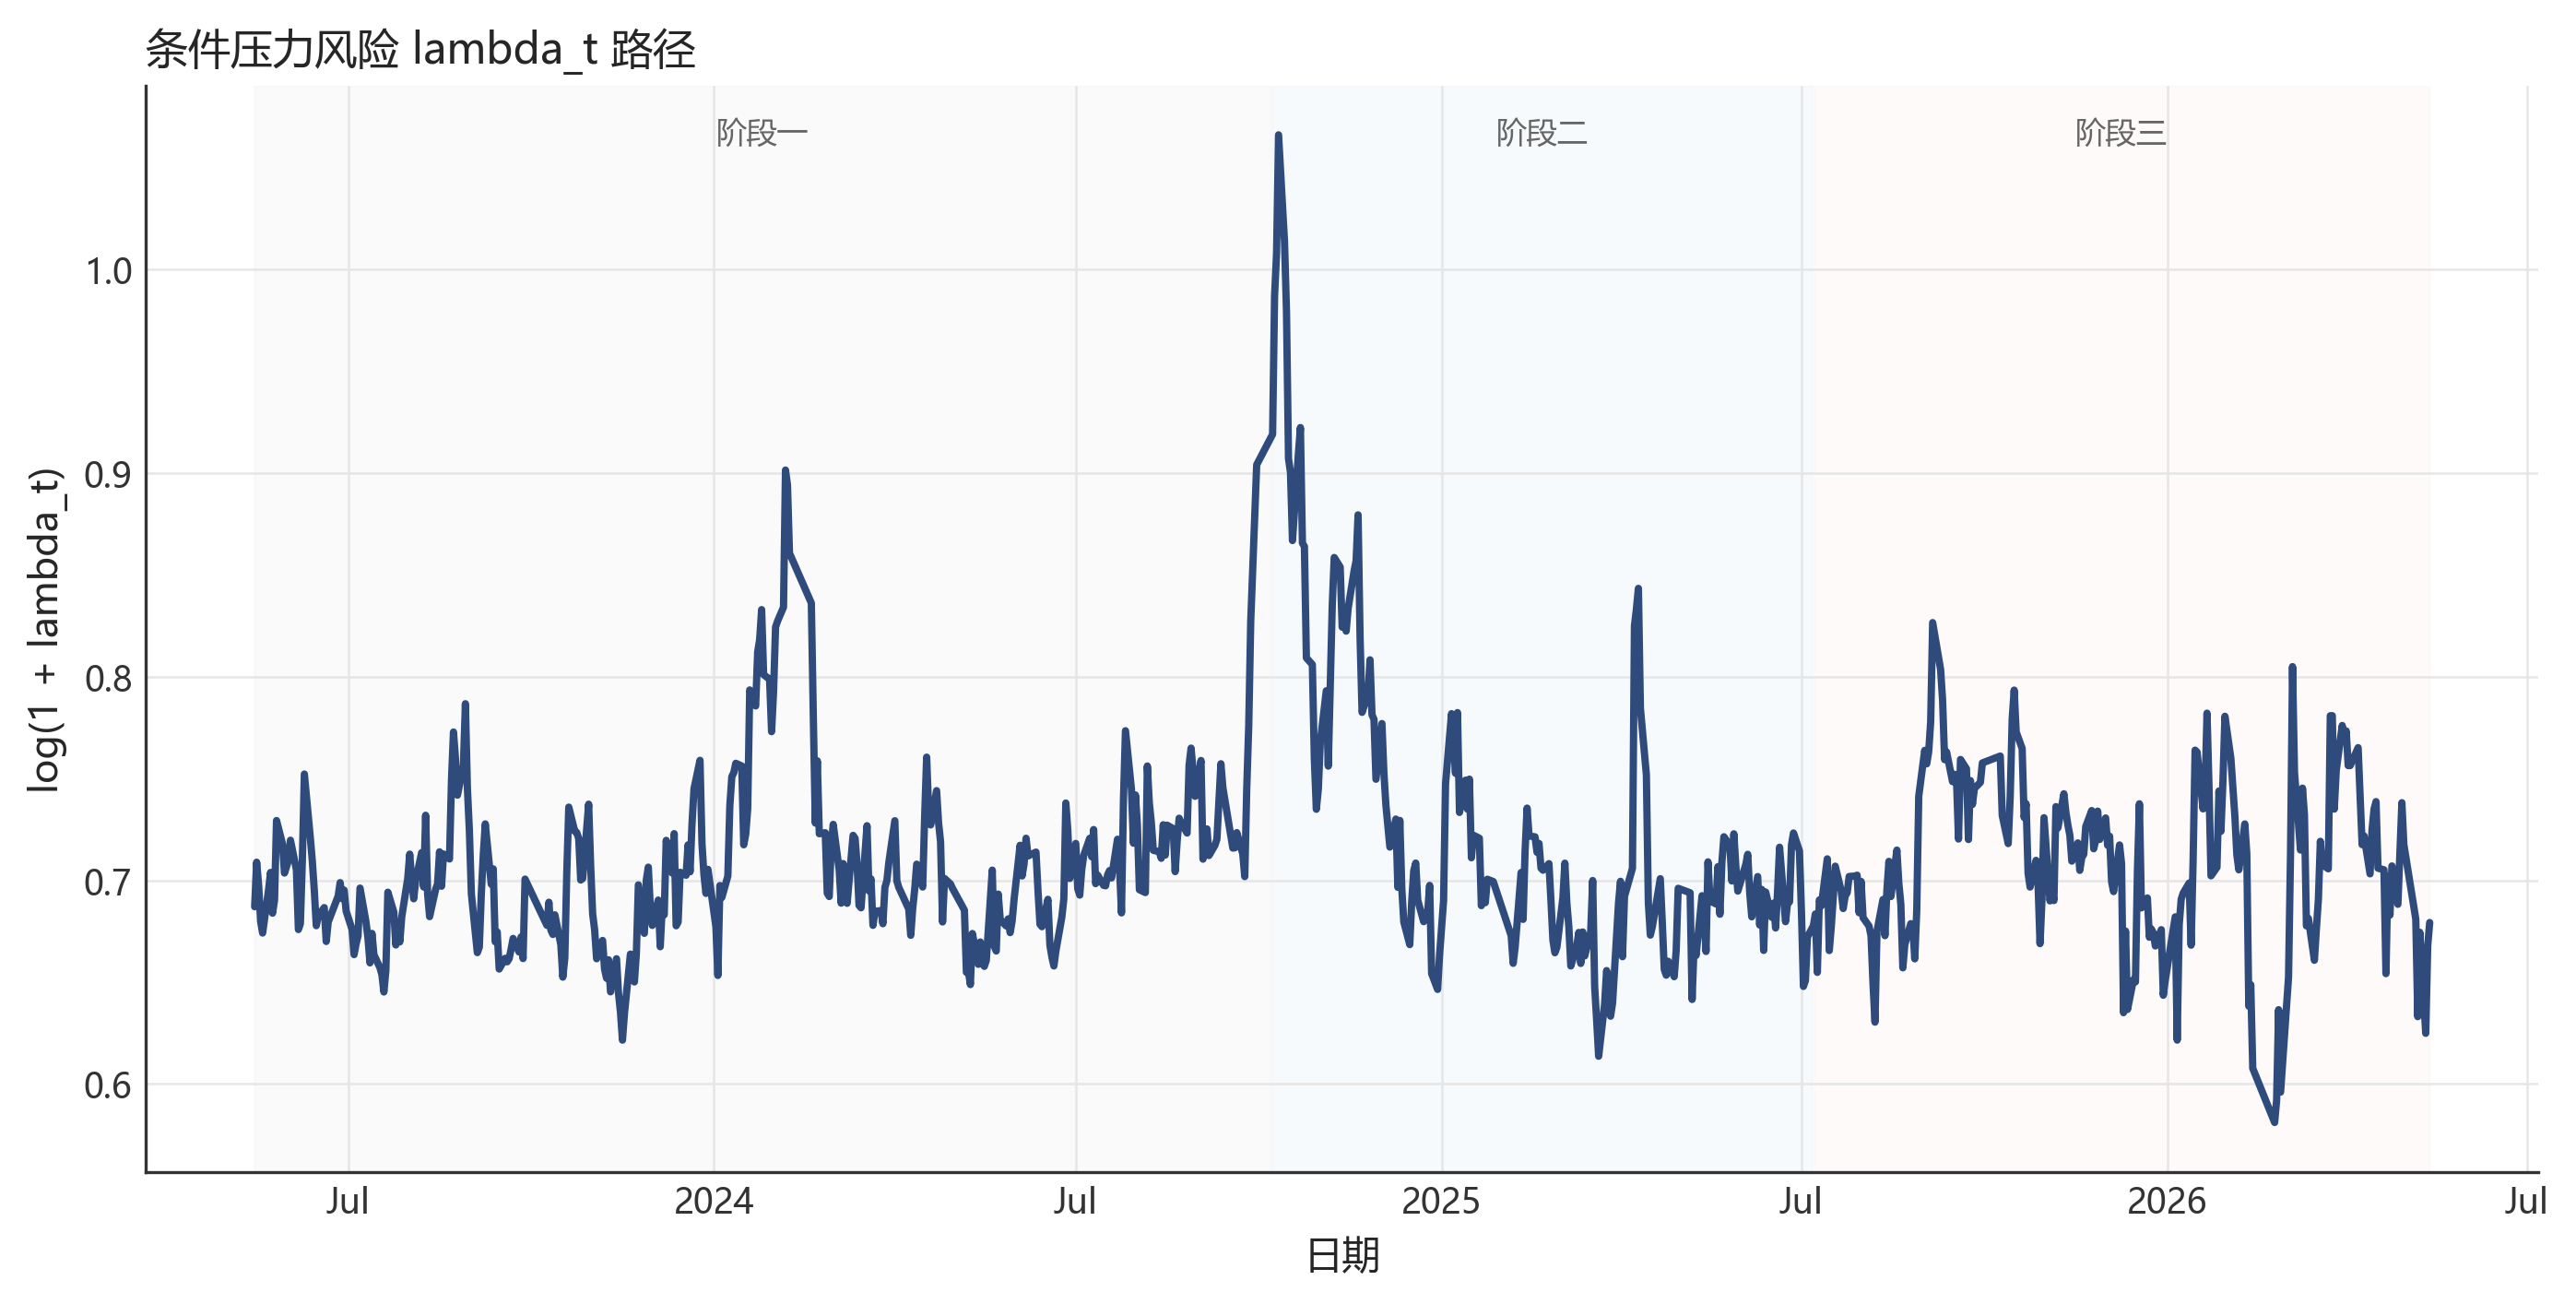
\includegraphics[width=0.92\textwidth]{figures/fig_rgarch_risk.png}
    \caption{RGARCH-CARR-SK 条件压力风险路径。该图用于刻画 MarketLSI 压力风险的阶段性聚集，而非收益率波动预测。}
    \label{fig:rgarch-risk}
\end{figure}

图 \ref{fig:rgarch-risk} 显示，条件压力风险 \(\lambda_t\) 在若干阶段出现明显抬升，且与 MarketLSI 局部峰值时段大体对应。这表明 realized pressure measure 能够为风险递推提供信息，MarketLSI 并非纯粹噪声，而具有一定的时间聚集特征。需要说明的是，该路径来自成交后市场状态构造的压力代理指标，不能直接观测买卖价差、挂单深度和订单恢复能力。

从 $\lambda_t$ 的经济意义看，条件压力风险水平的持续抬升表明 MarketLSI 的压力状态具有跨分钟的时间聚集性，而非逐分钟独立的随机波动。递推结构将已实现压力测度的历史信息延续至当前风险估计，使得高压力阶段的 $\lambda_t$ 不会因单个低压力分钟而骤然消散。这一聚集性特征正是使用时间序列动态风险框架而非静态截面描述的核心依据。

除条件压力风险水平外，RGARCH-CARR-SK 框架还允许通过动态高阶矩刻画压力创新分布的形状变化。由于本文的压力序列并非收益率本身，动态高阶矩不用于单独识别市场事件，而主要作为压力创新分布是否存在非对称性的诊断信息。基于此，图 \ref{fig:rgarch_dynamic_skewness} 报告动态偏度 \(s_t\) 的时间路径。

\begin{figure}[!htbp]
    \centering
    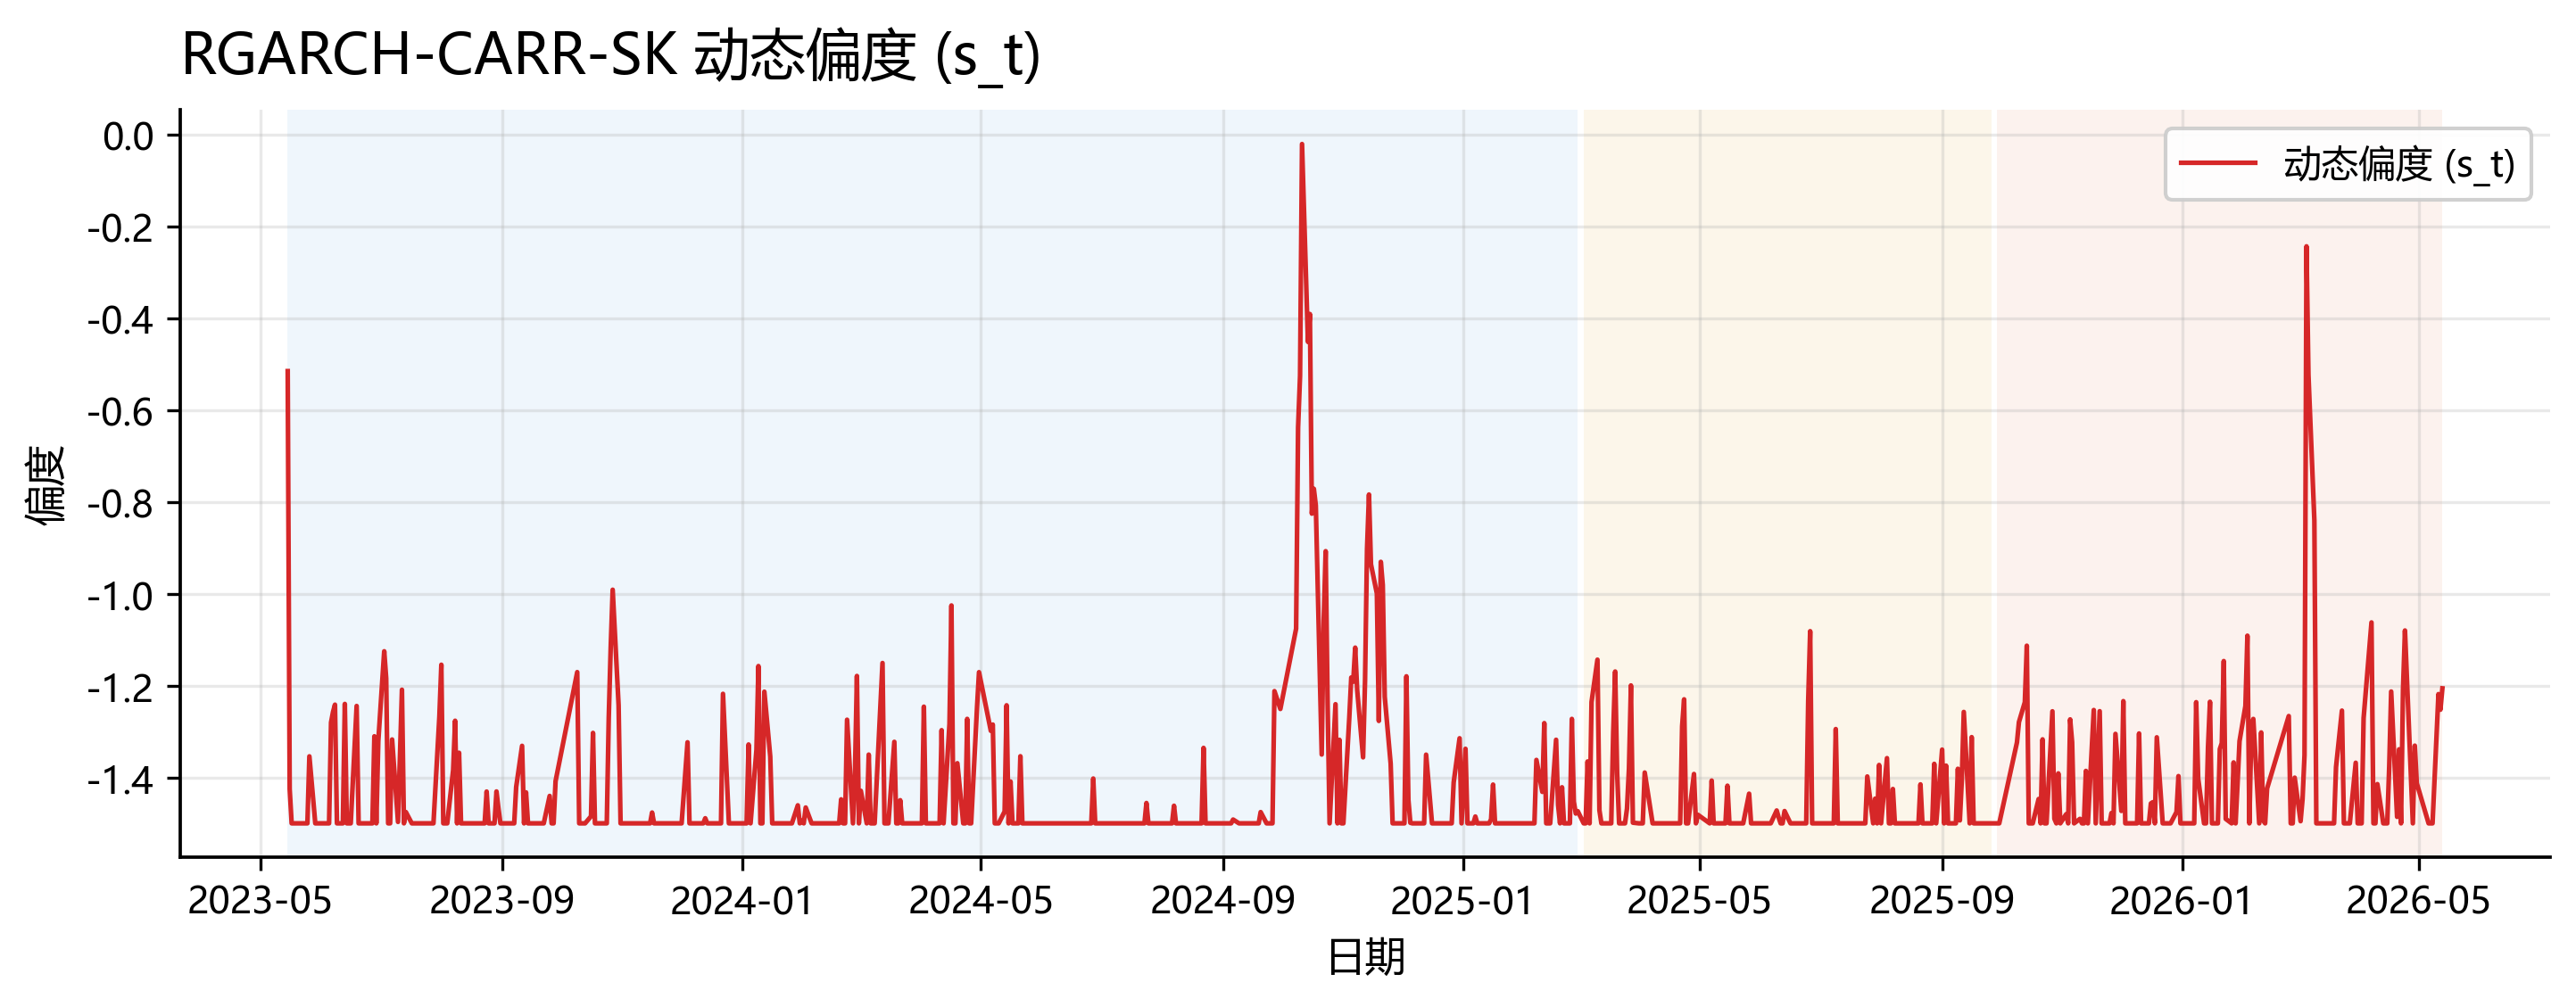
\includegraphics[width=0.92\textwidth]{figures/fig_rgarch_dynamic_skewness_refined.png}
    \caption{RGARCH-CARR-SK 动态偏度 \(s_t\) 路径。图中展示压力创新分布非对称性的时间变化，背景区间对应训练、验证与测试样本划分。}
    \label{fig:rgarch_dynamic_skewness}
\end{figure}

图 \ref{fig:rgarch_dynamic_skewness} 显示，动态偏度 \(s_t\) 在大部分时期位于负值区间，并在若干局部压力阶段出现向零附近的快速抬升。这说明 MarketLSI 压力创新不仅体现为条件风险水平的上升，也伴随创新分布非对称性的阶段性变化。结合图 \ref{fig:rgarch-risk} 的条件压力风险路径可以看出，RGARCH-CARR-SK 对本文的作用并不是直接预测收益率，而是从风险尺度和创新分布形状两个角度刻画短时压力状态的动态变化。

动态偏度的主要作用是辅助判断压力创新分布是否存在非对称性变化，而非作为独立核心结论；动态峰度在本样本中基本稳定于正态基准附近，不宜被解读为额外的厚尾动态证据，因此不作为后续讨论的重点。

与动态偏度不同，动态峰度 \(k_t\) 在本样本中基本稳定在正态基准附近。结合参数估计和模型边界约束，这一结果更适合作为模型诊断信息，而不宜被解释为额外的厚尾动态证据。因此，本文后续主要围绕条件压力风险 \(\lambda_t\)、动态偏度 \(s_t\) 以及 realized pressure measure 口径差异展开讨论。

为检验上述路径是否依赖 realized pressure measure 的具体口径，本文进一步比较 RV、RBV、MedRV 和 RMAD 四类测度下的拟合准则与样本外损失。

\begin{table}[H]
\centering
\caption{RGARCH-CARR-SK 拟合准则}
\label{tab:rgarch-fit}
\small
\begin{threeparttable}
\begin{tabular}{lrrr}
\toprule
realized measure & LLK & AIC & BIC \\
\midrule
RV & -169.822 & 365.64 & 418.62 \\
RBV & -198.783 & 423.57 & 476.54 \\
MedRV & -203.959 & 433.92 & 486.90 \\
RMAD & -553.492 & 1,133 & 1,186 \\
\bottomrule
\end{tabular}
\begin{tablenotes}[flushleft]
\footnotesize
\item 注：LLK、AIC 和 BIC 用于比较不同 realized pressure measure 下的样本内拟合表现。
\end{tablenotes}
\end{threeparttable}
\end{table}

\begin{table}[H]
\centering
\caption{RGARCH-CARR-SK 样本外损失}
\label{tab:rgarch-loss}
\small
\begin{threeparttable}
\begin{tabular}{lrrr}
\toprule
realized measure & R2LOG(validation) & R2LOG(test) & MAE(test) \\
\midrule
RV & 15.605 & 15.396 & 53.392 \\
RBV & 15.578 & 15.266 & 53.420 \\
MedRV & 16.855 & 16.693 & 53.378 \\
RMAD & 0.020 & 0.030 & 0.131 \\
\bottomrule
\end{tabular}
\begin{tablenotes}[flushleft]
\footnotesize
\item 注：R2LOG 为损失指标，数值越低越好。RMAD 的 R2LOG 明显低于其他测度，但该差异与测度尺度有关，因此正文使用表格报告而不使用线性尺度柱状图。
\end{tablenotes}
\end{threeparttable}
\end{table}


表 \ref{tab:rgarch-fit} 与表 \ref{tab:rgarch-loss} 表明，不同 realized pressure measure 会改变模型的拟合表现和样本外损失。RMAD 在 R2LOG 上表现较低，但该差异与测度尺度及压力序列构造有关。因此，本文不据此宣称 RMAD 在所有意义上绝对最优，而将其解释为风险路径对 realized pressure measure 设定具有敏感性。RV、RBV、MedRV 与 RMAD 四类测度在分布中心和尾部信息的处理方式上存在统计差异，进而使条件压力风险估计对测度口径较为敏感；这与高频波动文献中不同已实现测度对微观结构噪声具有不同稳健性的观点一致。

总体而言，RGARCH-CARR-SK 提供了本文第一层证据：MarketLSI 压力风险具有阶段性聚集特征，且风险路径对 realized pressure measure 的选择较为敏感。这一结果为后续 QVAR 的尾部分位传导分析和 SMARTBoost 的样本外预警检验提供了风险状态背景。

\FloatBarrier

\subsection{QVAR 尾部分位传导与压力测试}

RGARCH-CARR-SK 描述单一 MarketLSI 压力风险路径，而 QVAR 进一步考察 MarketLSI 与市场收益、市场波动、成交承接状态之间的条件分位联动。

表 \ref{tab:qvar-pinball} 报告 MarketLSI 方程在不同分位点下的样本外 pinball loss。

\begin{table}[H]
\centering
\caption{QVAR MarketLSI 方程样本外 pinball loss}
\label{tab:qvar-pinball}
\small
\begin{tabular}{lrrr}
\toprule
样本区间 & 分位点 & MarketLSI pinball loss & 观测数 \\
\midrule
validation & 0.10 & 0.0279 & 33,350 \\
validation & 0.50 & 0.0490 & 33,350 \\
validation & 0.90 & 0.0307 & 33,350 \\
validation & 0.95 & 0.0224 & 33,350 \\
test & 0.10 & 0.0270 & 33,350 \\
test & 0.50 & 0.0447 & 33,350 \\
test & 0.90 & 0.0303 & 33,350 \\
test & 0.95 & 0.0231 & 33,350 \\
\bottomrule
\end{tabular}
\end{table}


表 \ref{tab:qvar-pinball} 显示，\(q=0.95\) 在样本外 pinball loss 上表现较好，说明尾部分位模型能够捕捉 MarketLSI 高压力状态。中位数分位点与尾部分位点的表现差异说明，普通均值或中位数关系不足以概括尾部压力状态。值得注意的是，较低的尾部 pinball loss 反映的是模型对高压力状态的分位拟合能力，而非 MarketLSI 对市场压力的因果预测能力；QVAR 的作用定位于条件联动的描述性刻画，而不构成结构识别。

在拟合表现之外，本文进一步比较不同分位点下 MarketLSI 条件响应路径。

\begin{figure}[H]
    \centering
    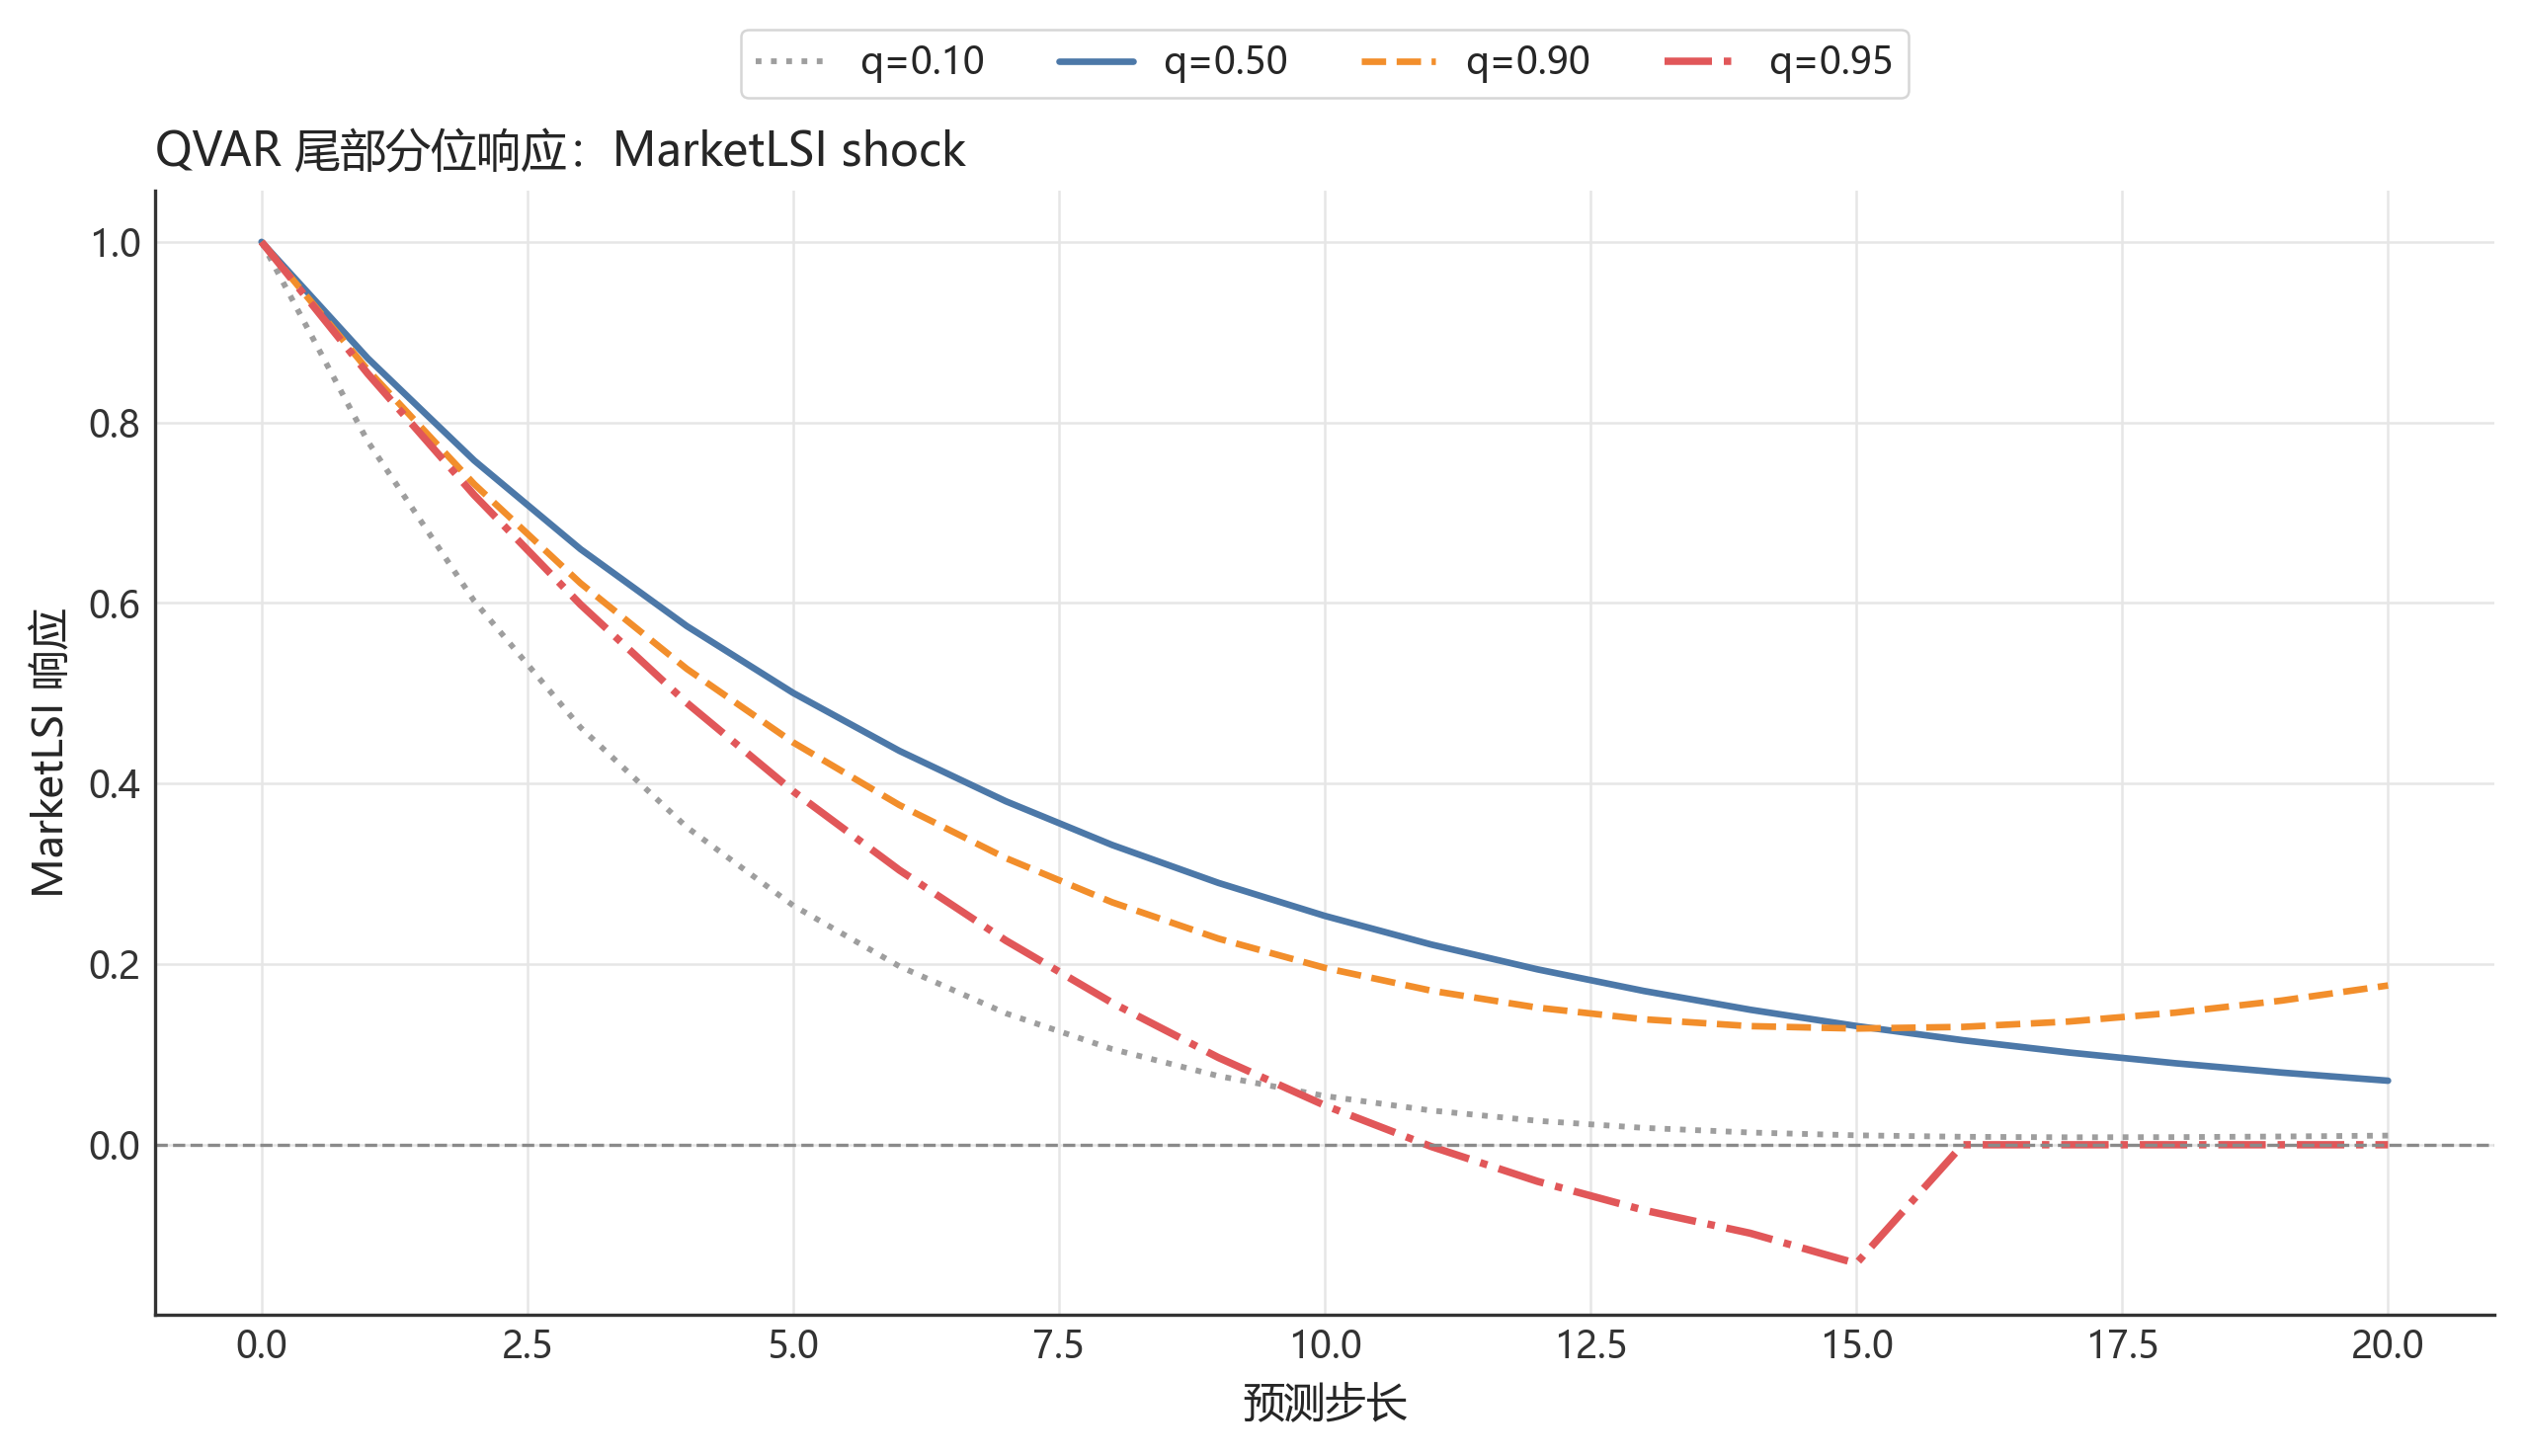
\includegraphics[width=0.90\textwidth]{figures/fig_qvar_response.png}
    \caption{QVAR 尾部分位响应。横轴为预测步长，曲线展示不同分位点下 MarketLSI 的条件响应路径；该结果反映尾部分位联动而非严格因果识别。}
    \label{fig:qvar-response}
\end{figure}

图 \ref{fig:qvar-response} 显示，不同分位点下的响应路径并不一致。中位数状态下的响应较为平滑，而尾部分位下的路径更容易出现非对称变化，说明短时压力状态具有尾部异质性。图中与 response 或 shock 相关的术语均应理解为标准化情景响应，不表示结构识别。这种尾部异质性还意味着，仅依赖中位数分位模型所提取的联动关系，会低估极端压力状态下市场变量之间的响应强度，从而使压力联动的实际程度被系统性低估。

为了使尾部分位响应具有更明确的经济解释，本文构造四类标准化情景。表 \ref{tab:qvar-scenarios} 给出对应设定。

\begin{table}[H]
\centering
\caption{QVAR 压力测试情景设定}
\label{tab:qvar-scenarios}
\small
\begin{threeparttable}
\begin{tabularx}{\textwidth}{p{0.18\textwidth}p{0.34\textwidth}Y}
\toprule
情景 & 标准化冲击 & 经济含义 \\
\midrule
市场急跌 & IndexRet = -2.0 & 模拟市场收益显著下行。 \\
波动放大 & IndexRV = +2.0 & 模拟指数波动显著上升。 \\
成交收缩 & MarketRelAmt = -2.0 & 模拟成交承接能力下降。 \\
复合压力 & IndexRet = -2.0, IndexRV = +2.0, MarketRelAmt = -2.0 & 模拟价格、波动与成交承接同时恶化。 \\
\bottomrule
\end{tabularx}
\begin{tablenotes}[flushleft]
\footnotesize
\item 注：冲击为标准化情景模拟，不代表严格因果识别。
\end{tablenotes}
\end{threeparttable}
\end{table}


这些情景均为标准化变量设定，只用于比较不同市场状态恶化时 MarketLSI 的相对响应，不代表真实外生事件识别。换言之，表 \ref{tab:qvar-scenarios} 的作用是为尾部分位联动提供可读的经济场景，而不是建立结构识别框架。

图 \ref{fig:qvar-stress} 进一步展示四类情景下 MarketLSI 的响应路径。

\begin{figure}[H]
    \centering
    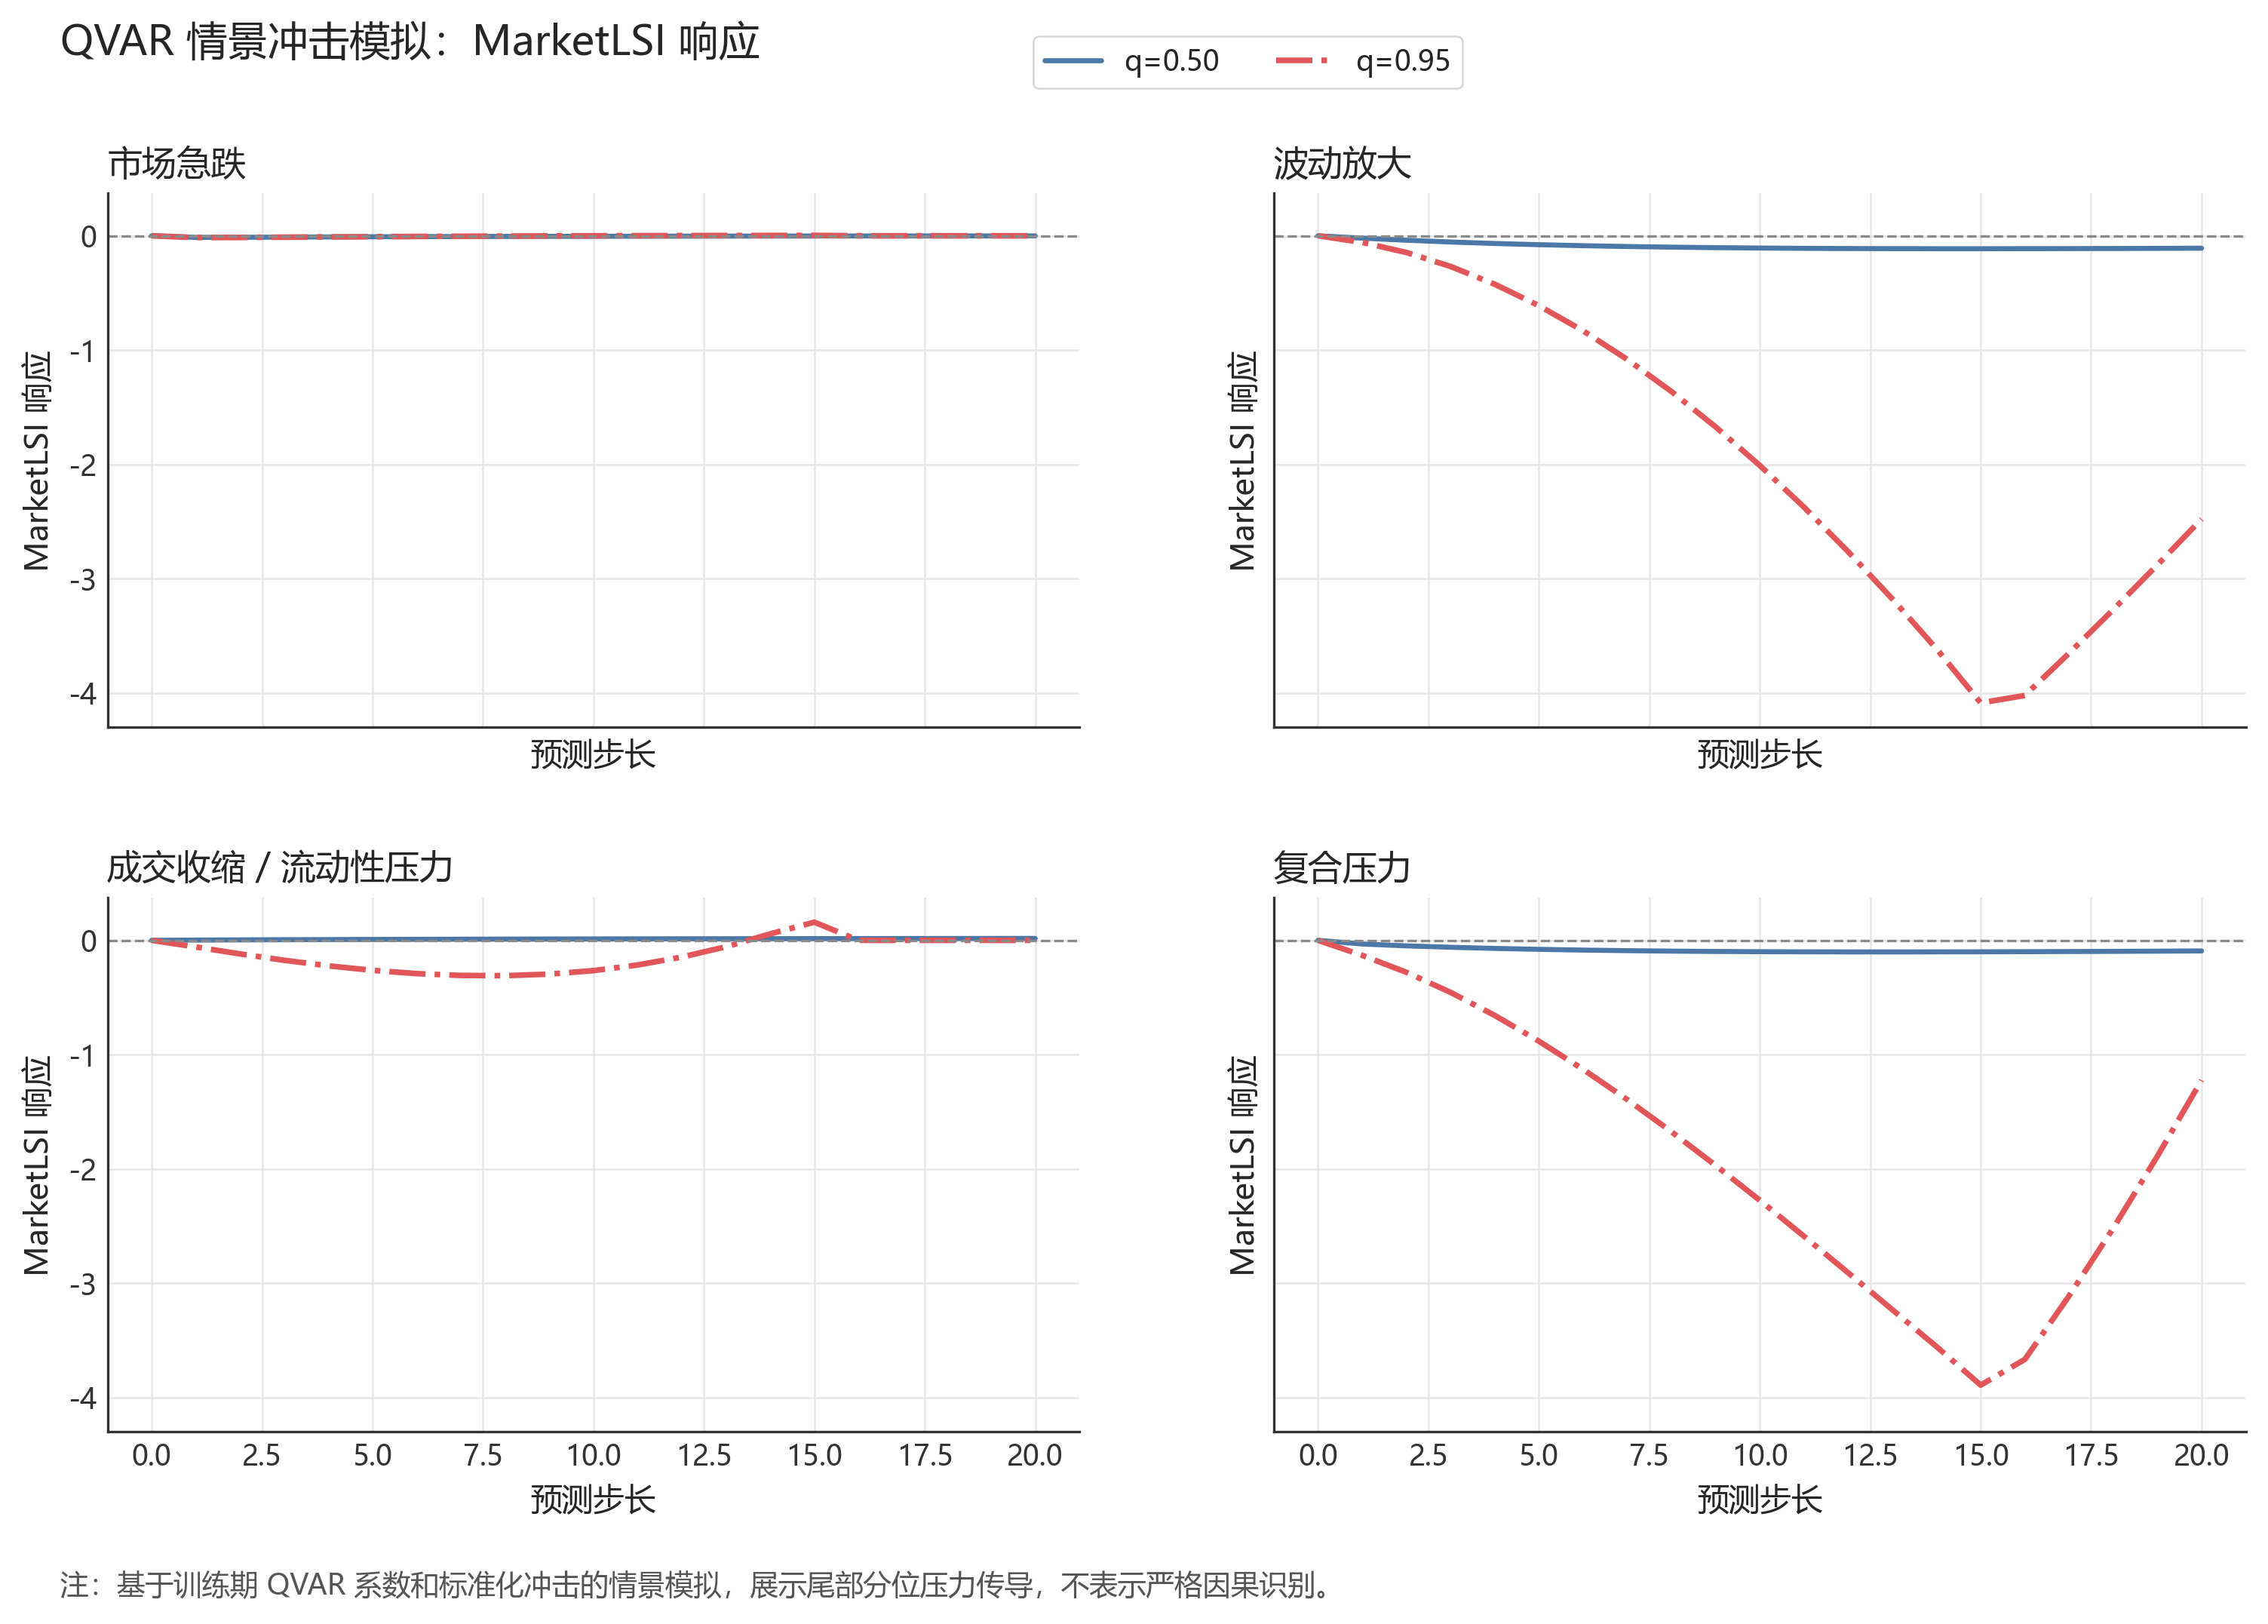
\includegraphics[width=0.94\textwidth]{figures/fig_qvar_stress.png}
    \caption{QVAR 四类压力测试情景。情景设定基于标准化变量，用于刻画不同市场状态恶化时 MarketLSI 的响应路径。}
    \label{fig:qvar-stress}
\end{figure}

图 \ref{fig:qvar-stress} 表明，波动放大和复合压力情景下 MarketLSI 响应更明显，说明短时压力并不只来自市场收益下跌，也与波动状态和成交承接能力变化有关。相比之下，单独市场急跌情景的响应相对较弱，提示分钟级压力预警应同时纳入波动和成交承接状态。复合情景下响应明显强于单一情景，进一步表明多维市场状态的协同恶化会放大压力联动；这与 LSI 指标同时纳入振幅、成交等多个维度的构造思路相互印证。

因此，QVAR 提供的是第二层证据：MarketLSI 与市场状态变量之间存在尾部分位联动，且压力响应在高分位状态下更明显。这一结果为后续机器学习模型加入 MarketLSI、IndexRV 和 MarketRelAmt 等历史状态特征提供了经验依据。

\FloatBarrier

\subsection{SMARTBoost 样本外预警结果}

SMARTBoost 是本文唯一正式的样本外预警模型。前两类模型提供风险刻画与尾部分位联动证据，而 SMARTBoost 直接检验历史分钟级状态变量能否预警未来 H5/H10 压力事件。

表 \ref{tab:smartboost-metrics} 报告 validation 和 test 样本上的主要预警指标。

\begin{table}[H]
\centering
\caption{SMARTBoost validation/test 样本外预警指标}
\label{tab:smartboost-metrics}
\scriptsize
\setlength{\tabcolsep}{3.8pt}
\begin{threeparttable}
\begin{tabular}{llrrrrrr}
\toprule
目标 & 区间 & 事件率 & PR-AUC & ROC-AUC & Top5率 & Top5召回 & Brier \\
\midrule
H10 & test & 5.80\% & 0.545 & 0.909 & 56.42\% & 48.60\% & 0.0435 \\
H10 & validation & 5.28\% & 0.528 & 0.901 & 52.02\% & 49.30\% & 0.0434 \\
H5 & test & 5.44\% & 0.603 & 0.930 & 59.30\% & 54.49\% & 0.0381 \\
H5 & validation & 5.06\% & 0.589 & 0.930 & 55.63\% & 55.01\% & 0.0403 \\
\bottomrule
\end{tabular}
\begin{tablenotes}[flushleft]
\footnotesize
\item 注：最终模型不含 CrossStress、Stress\_H5、Stress\_H10 或未来窗口派生变量；PR-AUC 和 Top5 结果是本文主要预警证据，ROC-AUC 仅作辅助参考。
\end{tablenotes}
\end{threeparttable}
\end{table}


测试集 H5 的 PR-AUC 为 0.603，H10 的 PR-AUC 为 0.545，均明显高于对应事件率。考虑到测试集事件率仅约 5\%--6\%，该结果说明模型并非简单追随基准概率，而是在高风险排序中提取到了有效信息。H5 的 PR-AUC 和 ROC-AUC 整体高于 H10，说明更短窗口内的压力延续性和历史状态信息更强。在高度不平衡的稀有事件预警任务中，PR-AUC 较 ROC-AUC 更难被多数类样本主导，因而是衡量排序能力的更敏感指标；上述结果表明模型具有超越随机排序的稀有压力事件识别能力。

由于压力事件具有明显不平衡性，本文进一步观察 PR 曲线而不是仅依赖 ROC-AUC。图 \ref{fig:sb-pr} 展示 validation 和 test 样本上的 PR 曲线。

\begin{figure}[H]
    \centering
    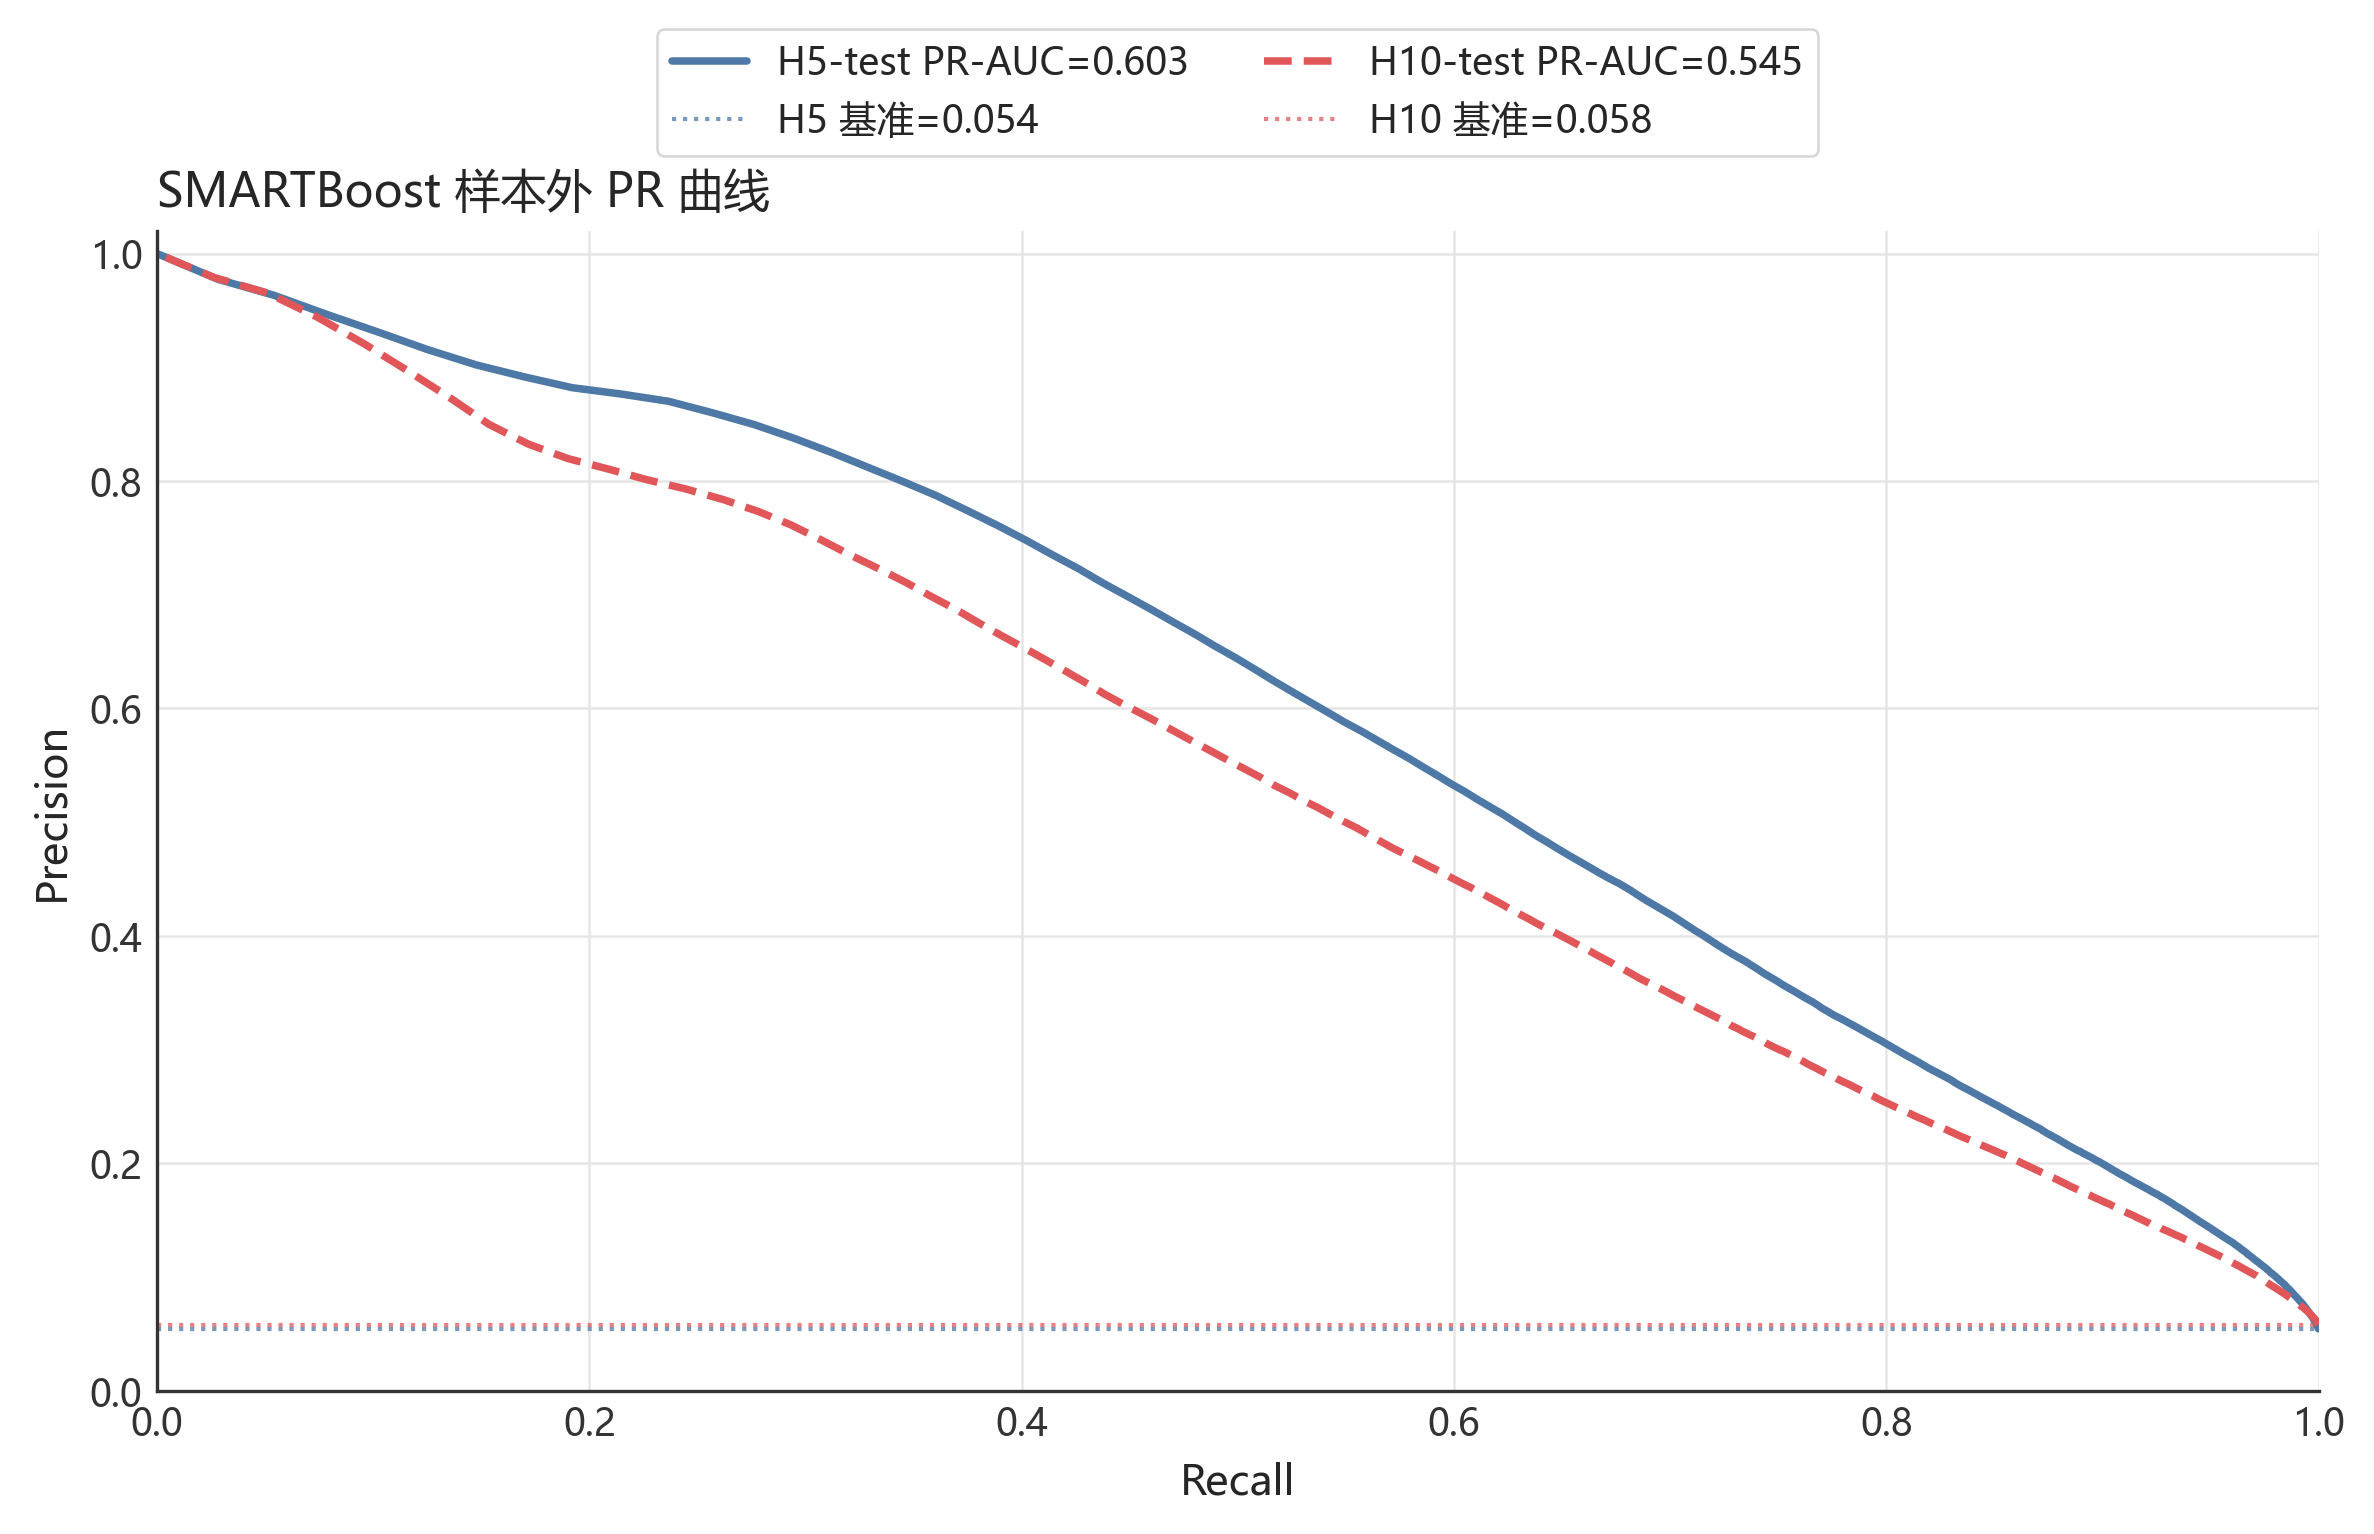
\includegraphics[width=0.88\textwidth]{figures/fig_sb_pr.png}
    \caption{SMARTBoost 样本外 PR 曲线。水平基准线表示对应样本的事件发生率，曲线越高说明模型越能在高风险排序中集中识别未来压力事件。}
    \label{fig:sb-pr}
\end{figure}

PR 曲线整体高于事件基准线，说明模型能够在较高预测概率区间集中识别未来压力事件。H5 曲线整体优于 H10，说明更短窗口内的压力延续性和历史状态信息更强。PR 曲线在较宽的召回率区间内持续高于水平基准线，意味着模型不只在极少数极端高风险样本上表现出色，而是在多个精确率—召回率权衡水平下均保持一定排序优势。

图 \ref{fig:sb-top5} 进一步考察预测概率最高的 Top 5\% 样本中真实压力事件的发生率。

\begin{figure}[H]
    \centering
    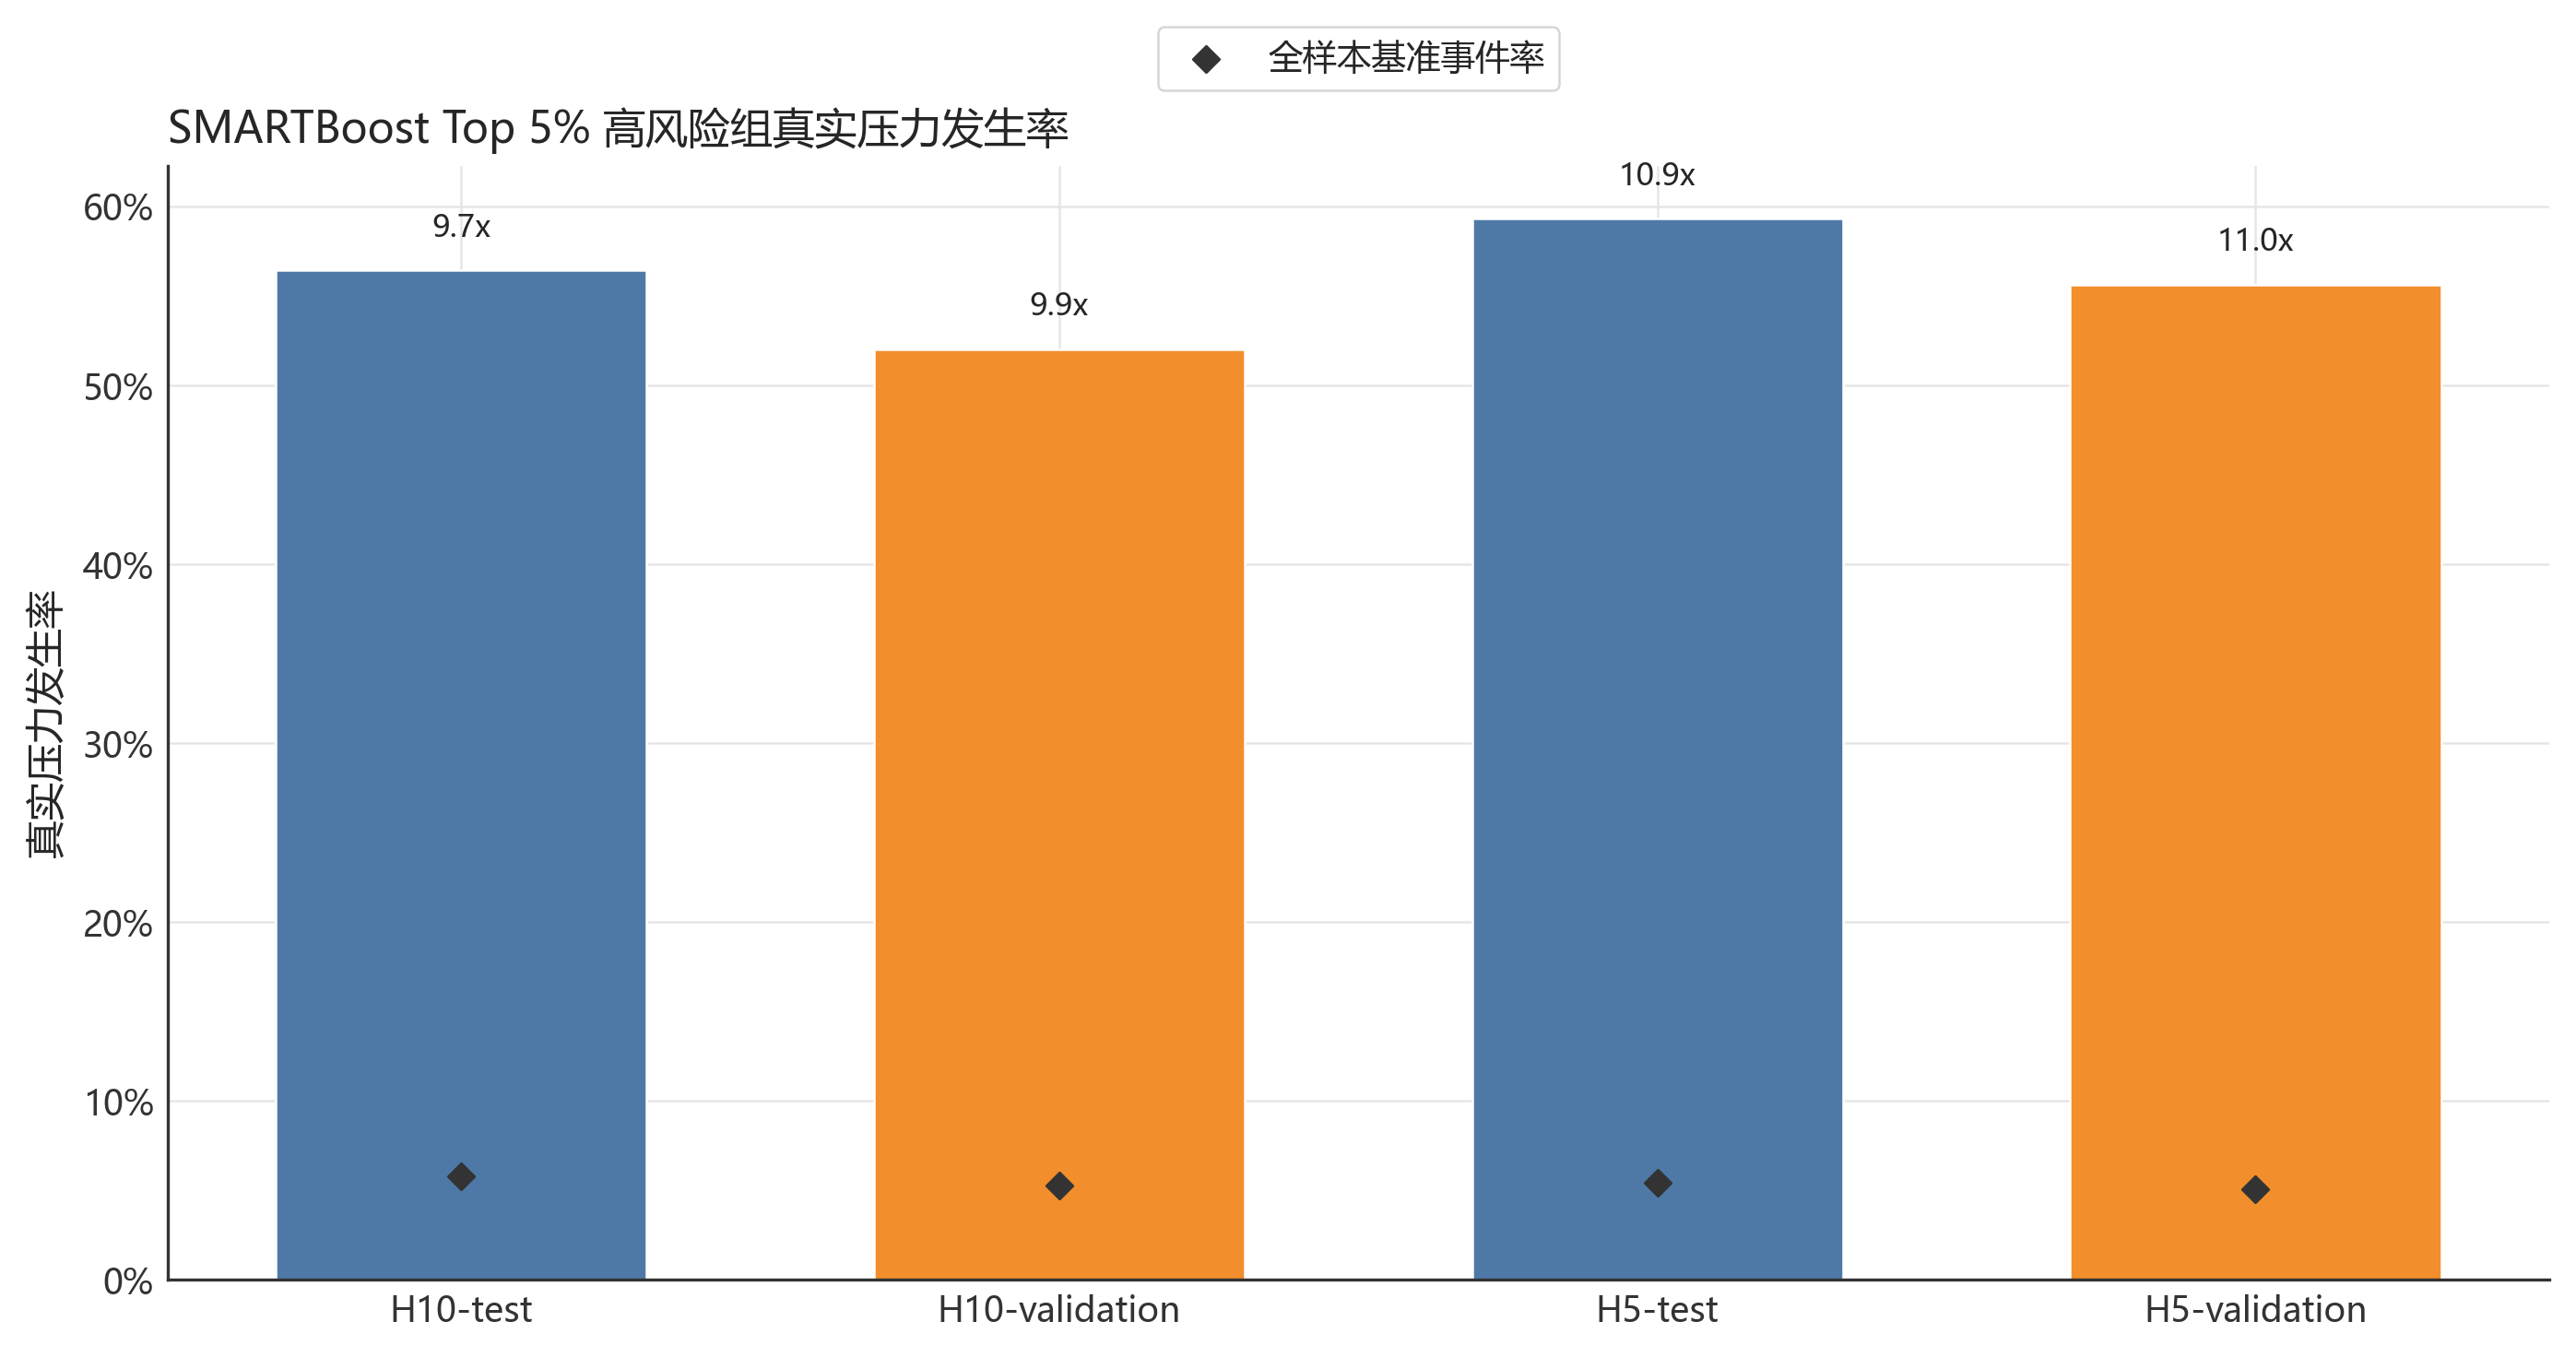
\includegraphics[width=0.88\textwidth]{figures/fig_sb_top5.png}
    \caption{SMARTBoost Top 5\% 高风险组真实压力发生率。柱状图展示 validation/test 与 H5/H10 组合下的高风险组命中表现，并与基准事件率对照。}
    \label{fig:sb-top5}
\end{figure}

Top 5\% 高风险组中的真实压力发生率显著高于样本整体事件率，lift 约为 10 倍。这是本文最直观的预警证据：模型不需要准确预测所有样本，而是能够将有限预警资源集中到最可能发生压力的少数样本上。

表 \ref{tab:smartboost-topk} 报告 test 样本中不同高风险分组的命中率与 lift，用于检验上述结论是否只依赖 Top 5\% 这一单一阈值。

\begin{table}[H]
\centering
\caption{SMARTBoost test 高风险组真实压力发生率与 lift}
\label{tab:smartboost-topk}
\small
\begin{threeparttable}
\begin{tabular}{lrrr}
\toprule
目标 & 高风险组 & 真实压力发生率 & lift \\
\midrule
H10 & 1\% & 85.71\% & 14.77 \\
H10 & 5\% & 56.42\% & 9.72 \\
H10 & 10\% & 38.54\% & 6.64 \\
H10 & 20\% & 23.74\% & 4.09 \\
H5 & 1\% & 89.41\% & 16.43 \\
H5 & 5\% & 59.30\% & 10.90 \\
H5 & 10\% & 39.26\% & 7.21 \\
H5 & 20\% & 23.56\% & 4.33 \\
\bottomrule
\end{tabular}
\begin{tablenotes}[flushleft]
\footnotesize
\item 注：Top-K 分组按预测风险从高到低排序得到；lift 为相对于 test 样本基准事件率的倍数。
\end{tablenotes}
\end{threeparttable}
\end{table}


表 \ref{tab:smartboost-topk} 显示，Top 1\% 到 Top 20\% 的高风险组均显著高于整体事件率；随着覆盖比例扩大，lift 递减属于风险排序任务中的正常现象。这一结果进一步说明 SMARTBoost 的优势主要体现为高风险排序，而不是对所有分钟样本进行同等精度的分类。在实践层面，高风险分组的价值在于面对有限监测资源时，能够将重点预警集中于最可能发生压力的少数时间点；因此，lift 较总体分类准确率更能反映模型的实际预警价值。

图 \ref{fig:sb-partial} 展示核心变量的 Partial Effects，用于解释主要特征如何影响预测概率。

\begin{figure}[H]
    \centering
    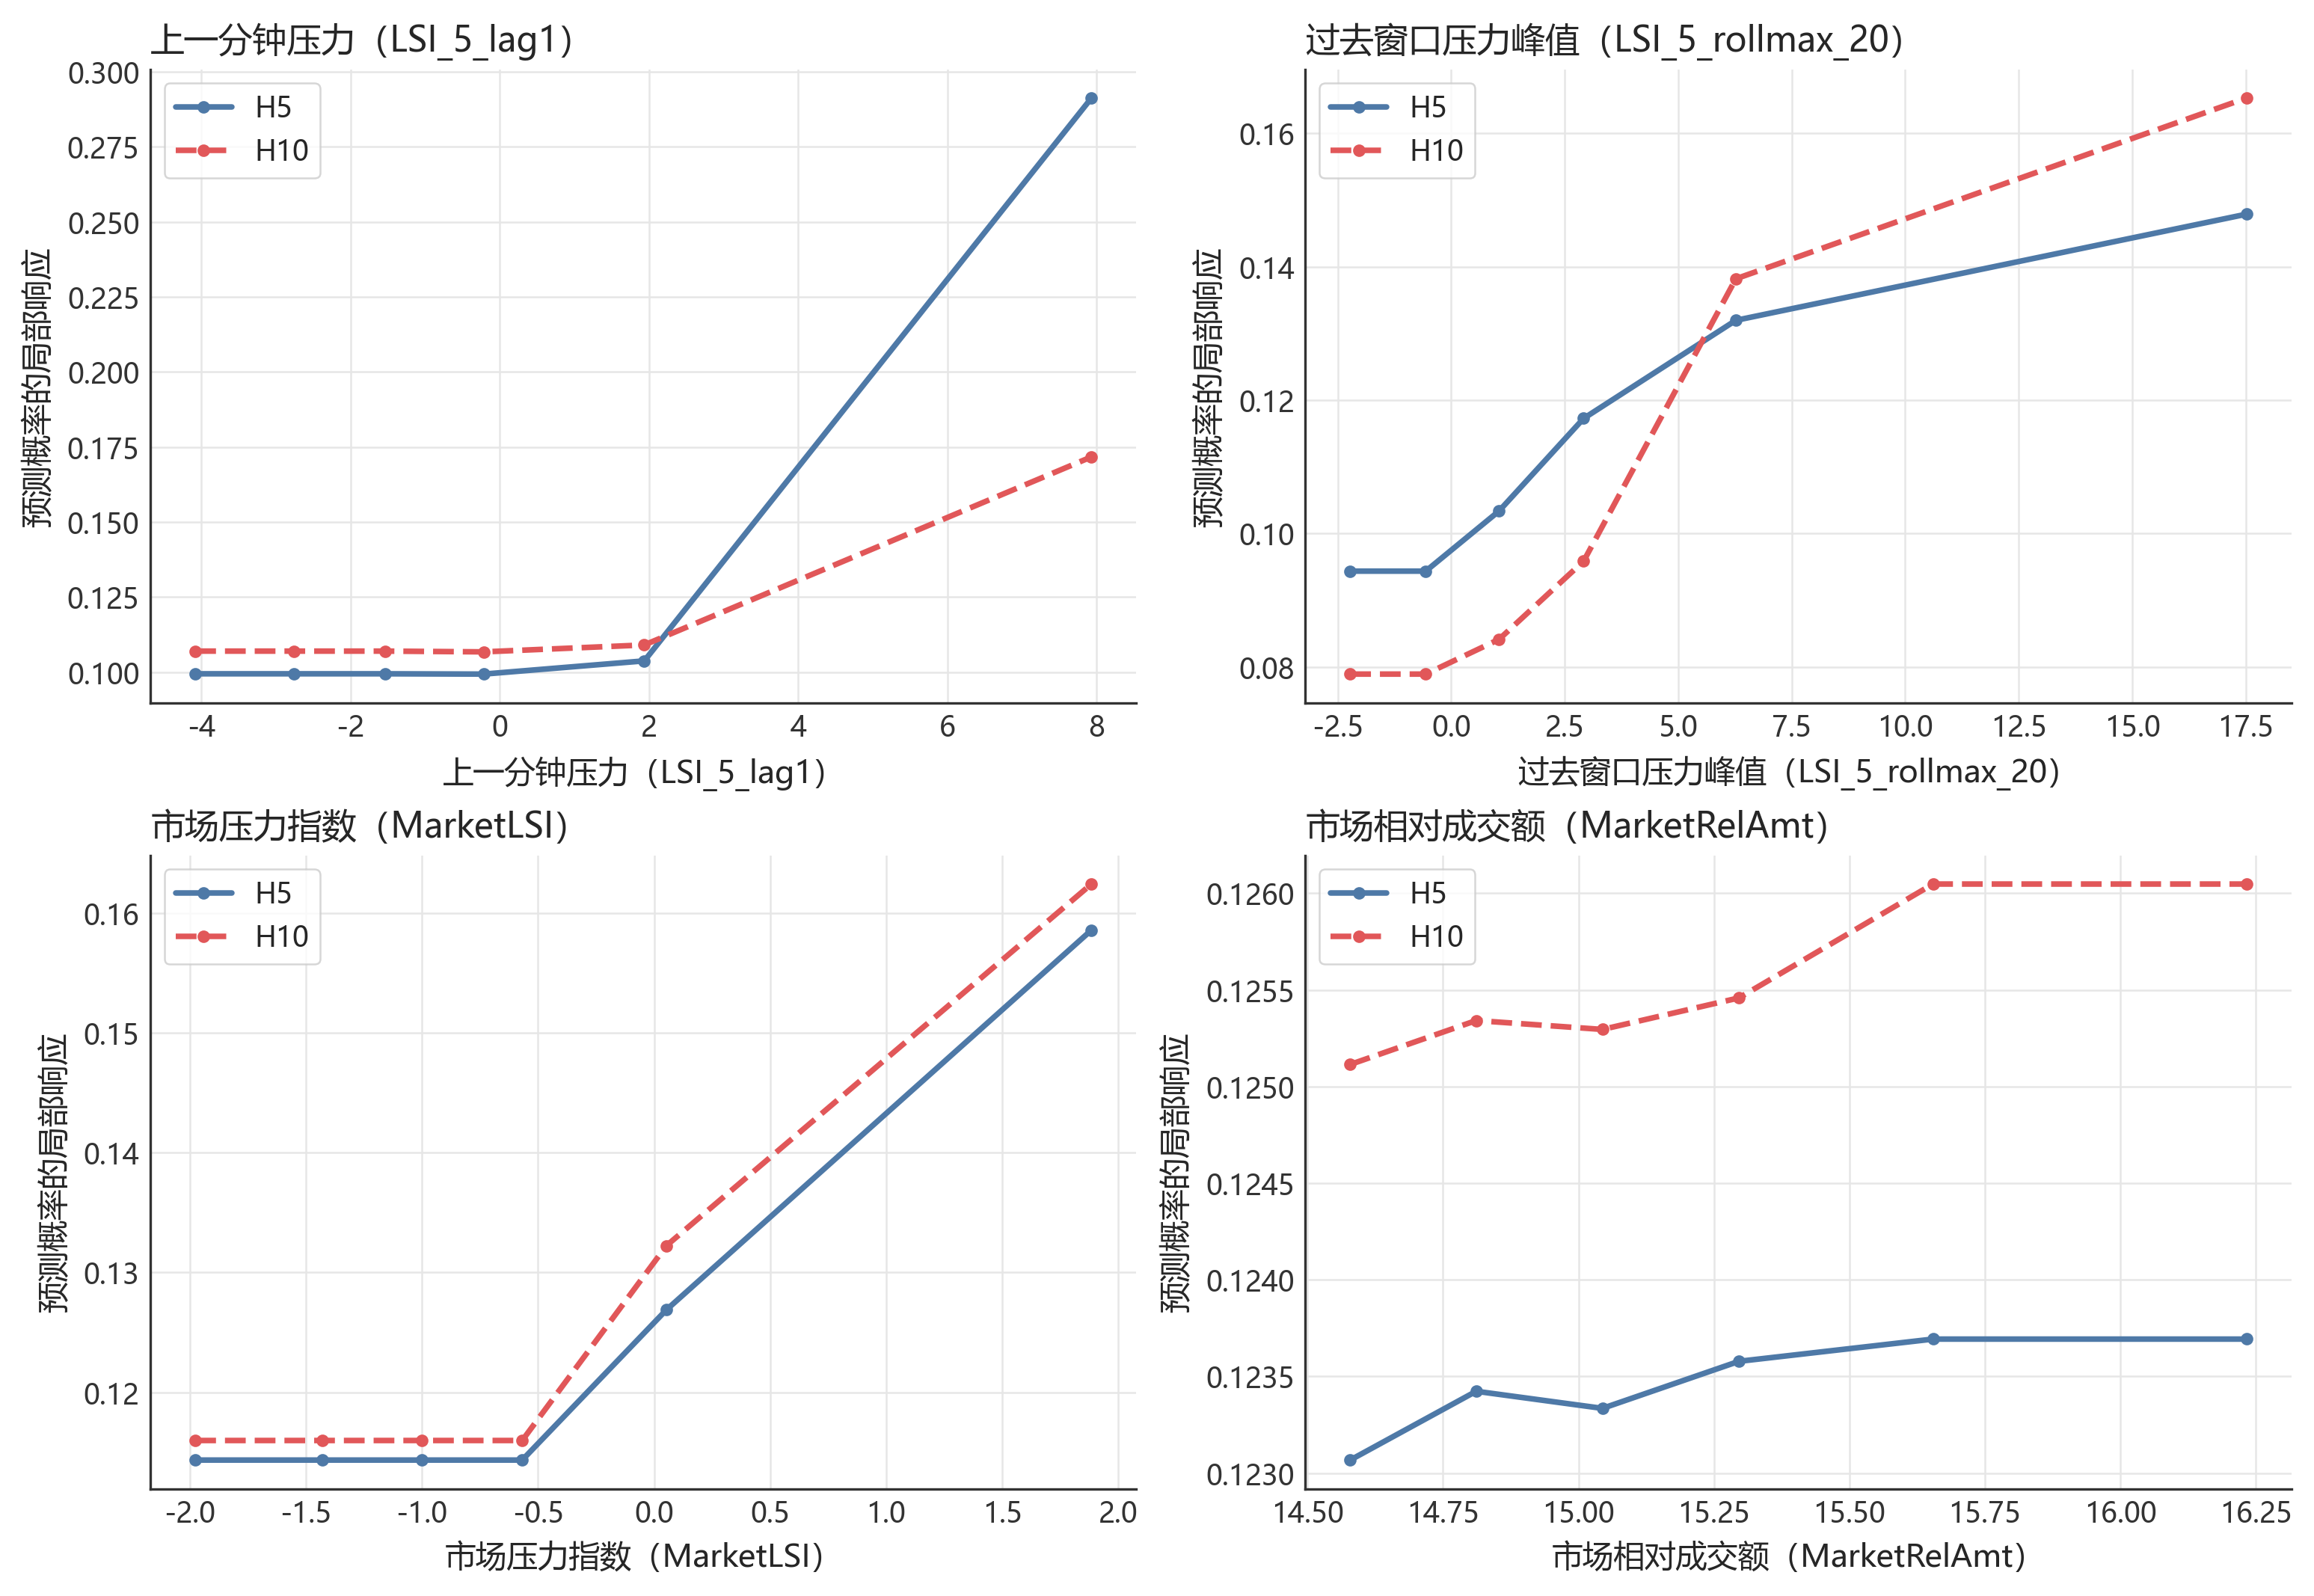
\includegraphics[width=0.90\textwidth]{figures/fig_sb_partial.png}
    \caption{SMARTBoost 核心变量 Partial Effects。横轴使用“中文说明 + 英文变量名”的形式，纵轴表示预测概率的局部响应。}
    \label{fig:sb-partial}
\end{figure}

Partial Effects 显示，上一分钟压力、过去窗口压力峰值和 MarketLSI 上升时，预测压力概率整体增加；MarketRelAmt 则反映成交承接状态的边际变化。该结果与 LSI 构造中的经济直觉一致，但仍应解释为预测模型的局部响应，而非因果效应。局部效应方向与 LSI 指标的构造逻辑相吻合，增强了机器学习预警结果的经济解释性，亦可间接验证模型提取的信息来自具有经济含义的高频状态变量，而非数据中的偶然统计关联。

最终预测特征不包含 Stress\_H5、Stress\_H10、FutureMaxLSI 和 CrossStress。所有特征均在预测时点或此前可观测，标准化参数和标签阈值仅来自训练期历史分布。因此，样本外表现可以解释为历史高频状态变量的预警能力，而不是未来信息泄漏带来的拟合结果。

SMARTBoost 提供的是第三层也是最直接的证据：在严格时间切分和防泄漏约束下，分钟级历史状态变量能够对未来 H5/H10 压力事件形成样本外风险排序。

\FloatBarrier

\subsection{三类证据链的综合解释}

RGARCH-CARR-SK、QVAR 和 SMARTBoost 的关系不是并列模型竞赛，而是递进证据链。RGARCH-CARR-SK 说明 MarketLSI 压力风险具有阶段性聚集，并且风险路径对 realized pressure measure 设定敏感；QVAR 说明这种压力状态与收益、波动和成交承接之间存在尾部分位联动；SMARTBoost 则检验这些历史状态变量能否真正形成样本外预警。

从研究问题看，本文的最终回答是肯定的：A 股分钟级市场状态信息能够对未来 5 分钟和 10 分钟短时流动性压力形成可验证预警。但这种结论有明确边界：LSI 是代理型压力指标，QVAR 是条件分位响应而非因果识别，SMARTBoost 是事件排序预警而非收益率预测。

\FloatBarrier
